%%%%%%%%%%%%%%%%%%%%%%%%%%%%%%%%%%%%%%%%%
% University/School Laboratory Report
% LaTeX Template
% Version 3.1 (25/3/14)
%
% This template has been downloaded from:
% http://www.LaTeXTemplates.com
%
% Original author:
% Linux and Unix Users Group at Virginia Tech Wiki 
% (https://vtluug.org/wiki/Example_LaTeX_chem_lab_report)
%
% License:
% CC BY-NC-SA 3.0 (http://creativecommons.org/licenses/by-nc-sa/3.0/)
%
%%%%%%%%%%%%%%%%%%%%%%%%%%%%%%%%%%%%%%%%%

%----------------------------------------------------------------------------------------
%	PACKAGES AND DOCUMENT CONFIGURATIONS
%----------------------------------------------------------------------------------------

\documentclass{article}

\usepackage[version=3]{mhchem} % Package for chemical equation typesetting
\usepackage{siunitx} % Provides the \SI{}{} and \si{} command for typesetting SI units
\usepackage{graphicx} % Required for the inclusion of images
\usepackage{natbib} % Required to change bibliography style to APA
\usepackage{amsmath} % Required for some math elements 
%\usepackage{url}
\usepackage{hyperref}
\usepackage{subcaption}
\usepackage{float}


\setlength\parindent{0pt} % Removes all indentation from paragraphs

%\renewcommand{\labelenumi}{\alph{enumi}.} % Make numbering in the enumerate environment by letter rather than number (e.g. section 6)

%\usepackage{times} % Uncomment to use the Times New Roman font

%----------------------------------------------------------------------------------------
%	DOCUMENT INFORMATION
%----------------------------------------------------------------------------------------

\title{Homework \#2 \\AES implementation \\[0.2em]\small{}CNS Course Sapienza} % Title and subtitle

\author{Riccardo \textsc{Prinzivalle}, 1904064} % Author name

\date{October 30, 2020} % Date for the report

\begin{document}

\maketitle % Insert the title, author and date

%----------------------------------------------------------------------------------------
%	SECTION 1
%----------------------------------------------------------------------------------------

\section{Homework Goal}

This homework contains a basic python implementation of AES algorithm. Throughout the work, it has been chosen to make a compromise: the implementation is in midpoint between complete Galois Field and precomputed look-up tables for every step. Both encryption and decryption are studied and implemented, then the operatives modes are implemente and finally it will illustrate a comparison with world known AES implementations.

\section{Encryption}
Before digging into the details of every operation performed, it is necessary to explain how the variables are stored in this implementation: the 4x4 state matrix is threated as single vector of 16 components, from which of course it is possible to build the matrix representation and viceversa, it was only a choice due to initial lack of knowledge of python language; every state block is a byte stored in hex values to simplify computations (as I discovered python stores hex values as int so in practice the bytes blocks are stored as int). Also the key is stored as an array of 16 bytes, and every bytes follows the same philosophy adopted for the state. \newline
AES encryption can be decomposed into a sequence of the following four big blocks:  

\begin{enumerate}
\begin{item}
Byte Substitution
\end{item}
\begin{item}
Shift Row 
\end{item}
\begin{item}
Mix Columns
\end{item}
\begin{item}
Key Addition 
\end{item}
\end{enumerate}

The following subsections contains implementation details and choices made to build the single blocks.

\subsection{Byte Substitution}

The byte substitution block is build by two fuctions, one perform the single byte substitution operation (\textit {subByteSingle}), while the other one (\textit {subByte}) performs the byte substitution to all the byte of the state calling the previous function for every single byte. The basic operation of single byte substitution is performing simply by looking to a prestored table which contains all the values for the 256 combinations of 8 bit contained in one byte. This method is more efficient and more simpler to implement with respect to performing all the operations needed in GF(256).

\subsection{Shift Row}

The shift row block is a simple function wich perform a left row shift for every row of the state matrix; since the state is sorted as a plain array, it s necessary first to build the row of the matrix from the array, then perform the row shift and finally substitute back in the state array the shifted value. As written in AES standard, the shift is of one byte more very time one new row is processed (first row has no shift while last row has a circular shift of 3 bytes). 

\subsection{Mix Columns}

The mix column block is based on an intermediate difficulty of implementation: the base idea is taken from \cite{10.5555/560131}, which is the central operation performed inside the \textit{mixcolumns} function. In order to perform it, it is necessary to construct the columns from the array state and in the end rebuild the state vector form the columns. The central operation is based on another function called \textit{xtime}, which together with the xor operations, is able to substitute all the GF operations. The xtime function implements the multiplication of the polynomial stored in the byte for x, its idea is taken from \cite{AESxtime} and since the algorithm works with a byte implementation, it is necessary to use the final end in the return of the function to truncate the byte after the left shift. \newline
To debug this section, I used the test vetors which can be found in \cite{AESmixcolumn}.

\subsection{Key Addition}

The key addition layer basically uses 3 functions in this implementation: \textit{keyAddition} perform the xor operation between the state and the subkey (the for is necessary to perform the operation bytewise, since the state is an array); \textit{roundKey} generates the subkeys needed at every iteration of AES while \textit{gFuntion} is an auxiliary function needed by \textit{roundKey}. \newline
The \textit{gFunction} corresponds to function \textit{g} of classical AES implementation, the shift and the byte substitution are based on previous functions or parts of them, while the xor operation is performed with a precomputed vector instead of computing at every round the specific byte to xor. In this way, the implementation is more efficient and simpler.\newline
The \textit{roundKey} function first joins 4 bytes at a time of the key in order to work with words, then it needs the auxiliary \textit{gFunction}, then it performs the four cascaded xor and finally it rebuild the byte based key from the word.\newline
To debug this section, it has been used a step by step subkey generation that can be found in \cite{AESsteps}.   

%----------------------------------------------------------------------------------------
%	SECTION 2
%----------------------------------------------------------------------------------------

\section{Decryption}

The decryption part of AES is simpler than encryption since it is possible to reuse at least the key addition layer; based on implementation choices, as those mades in this homework, it is possible to reuse also the \textit{mixcolumn} idea in its inverse. The decryption is less efficient than its counterpart since it generates the subkeys at every round instead of generating it once and storing it, this has been chosen to speed up the implementation.
 
\subsection{Mix Columns Inverse}

The inverse of \textit{mixcolumns} reuses part of its direct function together with a precomputation: the columns are preprocessed (fig. \ref{fig:preprocessing}) and then they are elaborated by the \textit{mixcolumns} core (fig. \ref{fig:core}). All the matematical details on this choice can be found in chapter 4 of \cite{10.5555/560131}. 

\begin{figure}[H]
\centering
\begin{subfigure}{.54\textwidth}
  \centering
  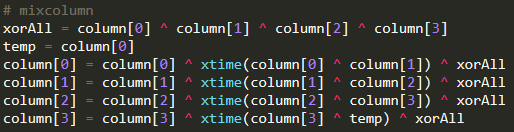
\includegraphics[width=1\linewidth]{images/mixcolumn.png}
  \caption{Core}
  \label{fig:core}
\end{subfigure}
\begin{subfigure}{.35\textwidth}
  \centering
  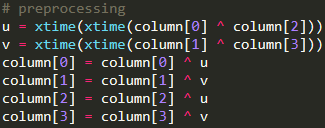
\includegraphics[width=1\linewidth]{images/preprocessing.png}
  \caption{Preprocessing}
  \label{fig:preprocessing}
\end{subfigure}
\caption{Mix columns base functions}
\label{fig:MixColumns}
\end{figure}

\subsection{Shift Row Inverse}

This blocks perform the row shift to the right, in order to reverse the \textit{shiftRow} operation. As before, from state it builds the necessary rows and at the end the state is rebuilt from each rows. In order to reverse the direct operation, the first row is not shifted while the others receive successive shift till the third row which undergoes a right shift of three elements.

\subsection{Byte Substitution Inverse}

This layer perform the inverse operation of Byte Substitution; it is based on two functions: \textit{subByteInv} is just a wrapper to call the base function on every byte of the state; \textit{subByteSingleInv} instead is the base funtion which performs the inverse Byte Substitution based on the inverse table seen before in the \textit{subByteSingle}.
 
%----------------------------------------------------------------------------------------
%	SECTION 3
%----------------------------------------------------------------------------------------

\section{Operation Modes}

\begin{tabular}{ll}
Mass of empty crucible & \SI{7.28}{\gram}\\
Mass of crucible and magnesium before heating & \SI{8.59}{\gram}\\
Mass of crucible and magnesium oxide after heating & \SI{9.46}{\gram}\\
Balance used & \#4\\
Magnesium from sample bottle & \#1
\end{tabular}

%----------------------------------------------------------------------------------------
%	SECTION 4
%----------------------------------------------------------------------------------------

\section{Real World Standard Comparison}

\begin{tabular}{ll}
Mass of magnesium metal & = \SI{8.59}{\gram} - \SI{7.28}{\gram}\\
& = \SI{1.31}{\gram}\\
Mass of magnesium oxide & = \SI{9.46}{\gram} - \SI{7.28}{\gram}\\
& = \SI{2.18}{\gram}\\
Mass of oxygen & = \SI{2.18}{\gram} - \SI{1.31}{\gram}\\
& = \SI{0.87}{\gram}
\end{tabular}

Because of this reaction, the required ratio is the atomic weight of magnesium: \SI{16.00}{\gram} of oxygen as experimental mass of Mg: experimental mass of oxygen or $\frac{x}{1.31}=\frac{16}{0.87}$ from which, $M_{\ce{Mg}} = 16.00 \times \frac{1.31}{0.87} = 24.1 = \SI{24}{\gram\per\mole}$ (to two significant figures).

%----------------------------------------------------------------------------------------
%	BIBLIOGRAPHY
%----------------------------------------------------------------------------------------

\bibliographystyle{abbrv}

\bibliography{sample}

%----------------------------------------------------------------------------------------


\end{document}